%\addcontentsline{toc}{chapter}{Development Process}
\chapter{Design}
The following section will cover the final design of the project, initial design can be seen in the Design Specification. The original design was completed when only a small amount of research had been completed and not all avenues of interest had been explored. Due to this good comparisons can be made between the two making it easy to highlight the areas of the design where large changes were made. The design covered is the cumulative output of the Design by Feature element in the process. This means some changes were still made during the implementation phase but those will be discussed in the relevant section.
 \newpage
\section{Support and Development Tools}
\subsection{Development Environment}
During the initial phases of development and prototyping Eclipse and the Android Development Tools\cite{adt} plug in were used to help develop the application, this was due to the developer having experience with this platform and the code being sampled from other projects was also built within this platform. However not long after initial prototyping and tech spikes had started to take place the decision was made to swap over to Android Studio and develop from there. Most of the decision comes down to personal preference but there are definitely good justifications to swap, personal preferences included appearance and responsiveness as well as easy to use features such as inbuilt git support and intuitive interfaces. 

One major contributing factor was the initial hassle in updating the ADT to their latest versions, this process alone took hours of research and tinkering to get fully working. During this time it was discovered that Google had stopped support for Eclipse ADT and would be focusing on the now fully released Android Studio\cite{as}. A decision was made, based on the advice from the Android API and other sites, to move over to Android Studio as it would quickly surpass Eclipse ADT with some features already being far more helpful.

One key feature that was seen as a bonus when compared to ADT was the interface editor, while this is present in the Eclipse version the process in Android Studio seemed much more responsive and seemed to give a clearer idea of what XML was being written to support the graphical changes. While nearly all interface development was completed using pure XML sometimes moving elements using the graphical layout gave good suggestions on exactly how a set layout could be achieved. While the code produced by this could sometimes be messy and convoluted it could also be cleaned up and improved. 

Some of the choice to move over was also personal opinion of the developers, with so much time having to be spent in the IDE it had to be at least a suitable experience. After past experience with Eclipse and ADT causing issues due to freezing and crashes the supposedly much more stable AS was worth adapting to. AS also seemed to provide a much fuller auto complete feature, suggestions would be made sometimes within a single letter of a word being typed out, normally correct suggestions. Once used to this process code could be written up slightly quicker making the experience overall more enjoyable and productive. Overall the experience with AS was that it was far less cumbersome and much more enjoyable than  Eclipse ADT. While currently there may not be huge differences the ones included were very helpful, the implementation of Gradle\cite{gradle} meant single lines could be used for the inclusion of dependencies and possible libraries. Easy inclusion like this meant that it was a lot more appealing to try out libraries and see what they added to the project. While Gradle provides many benefits not all were made of use within the project. 

A final reason for choosing Android Studio was that after seeing various comments on Android discussion boards it became obvious that it was quickly becoming the industry standard, unsurprisingly due to the lack of support for Eclipse ADT. Adapting to AS seemed the most logical decision, made easier by its sleek appearance and performance. 
\subsection{Version Control}
Version control was an easy problem to solve, as standard GitHub was used to upload versions of code and documents allowing the history of changes to be made and development easily tracked. It also meant that in future the project could easily be open sourced through the changing of the privacy settings on the repository. Using GitHub also meant that even when on the move developers could check the code base through the website to see if potential solutions could possibly be implemented. 

One alternative to GitHub which was considered was BitBucket, BitBucket provided unlimited private repositories and a desktop client which could have been of a fair amount of use. However looking at reviews and the general design, the developer decided that while there were benefits in using BitBucket over GitHub, they did not really apply to the project due to its small size. In future if the project was undertaken by a larger team, or the developer was part of a larger team for a seperate project, BitBucket could be heavily considered due to its unlimited private repositories as standard. 

Having the code stored off site as such also provides a range of benefits to the developers. It mostly frees up the developers to not worry about breaking any code, back ups from various times are all available with the ability to roll back to them with minimal effort. It also meant that the code was always safe, once the code had been moved to the GitHub servers its available for the future, no need to worry about corrupt drives or other similar issues. 

GitHub also provides a simple and easy to use graphical interface as an alternative to the command line interface. This interface was sufficient for the project being completed with only a few clicks allowing for the new code base to be committed and pushed to the on line version. While this may not seem a major benefit it still freed up some time and overall made the task of version control slightly more enjoyable. 

An alternative to using GitHub for version control and code backup was either storing backups externally using flash drives and external hard drives or using the file store given to students by the University. However the benefits provided by these were more than covered by what GitHub provided, it was also decided that there was a minimal chance of losing any data stored through GitHub while it was possible that we could lose access to the file store for prolonged periods of time without prior notice. This has been previously experienced and was not something that the developer wanted to risk.

Without version control it would be possible to completely lose track of what had changed, as well as losing the project as a whole. Storing everything locally is extremely bad practice as any amount of extenuating circumstances could lead to either the loss or damage of the computer that the information is stored on. Furthermore GitHub provided statistics on when most commits were made and exactly what was committed, this allowed for estimations on not only how long a feature would take to develop based on what time had currently passed, but how long a future feature would take based on its complexity compared to past features. This meant that during development a fairly tight schedule of development was set out and mainly adhered by.
\section{Overall Architecture}
Initial design for the project was very broad becoming more focused over development time. With the Design Specification it is possible to see the first properly documented steps in preparing for the development time within the project, however other initial steps were taken first to help build a design from. At the start of the project a very abstract set of diagrams were drawn up to describe the desired boundaries for the project, this was mainly as a guide for further development but aids in demonstrating the vision of the project from the start. While these were drawn up on paper the digitized version will follow, it can be seen that the diagram is essentially a flow diagram that only involves the Activities used in the Android application. No screen details are given just the links between them, this has changed significantly over development but the basic blocks can be seen here. A link can be seen between Route Plotter and Route Display, this was to represent the output from one being compatible with the other. \\
\begin{figure}[h]
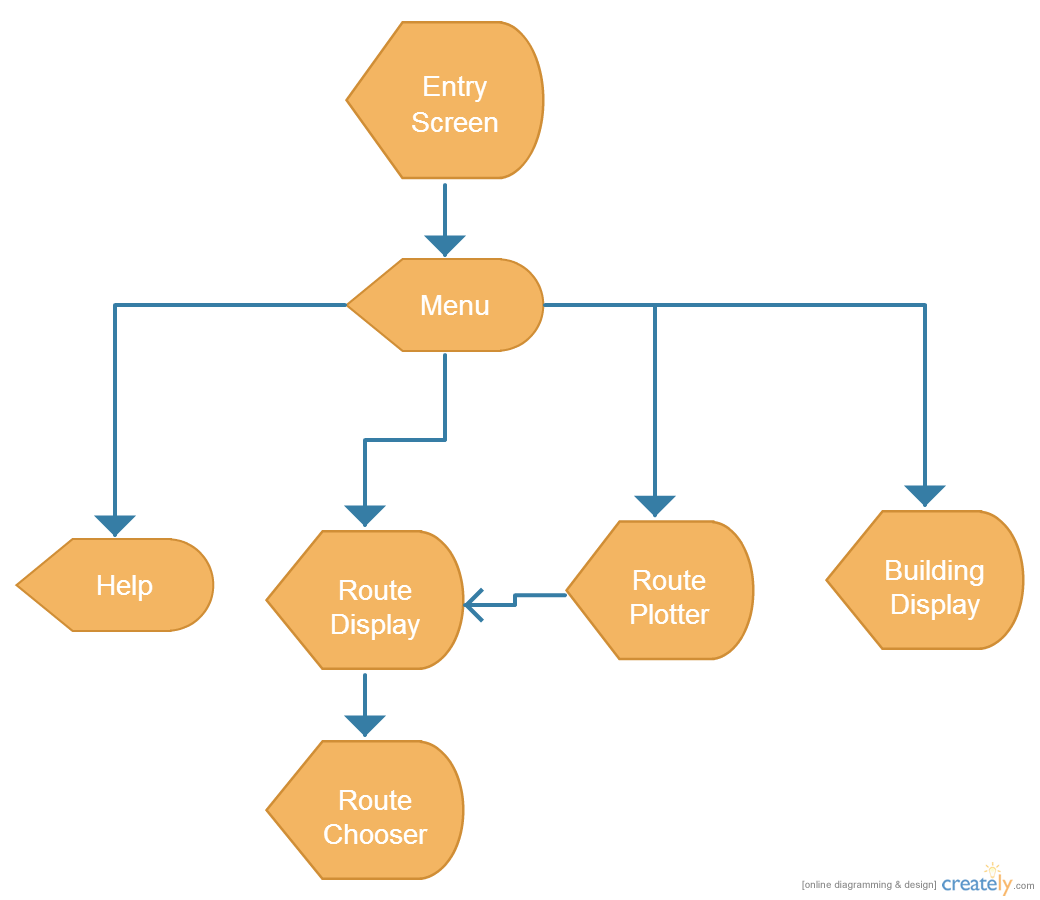
\includegraphics[scale=0.30]{Chapter2/screen.png}
\caption[Screen Flow]{Depiction of links between screens including some data compatibility.}
\end{figure}

\newpage
\subsection{Class Diagram and Justification}
The final Class Diagram represents what was thought to be the final representation before the Build Feature segment in the process, during implementation some changes were made but the class diagram is a good representation of how the program actually works. Justification of the design will follow with diagram afterwards. 
\subsubsection{Justification}
In this diagram the Menu Activity serves as an entry point into the program, in production it was always intended to have a simple screen before this, however for the case of the class diagram representing it is non informative as it does nothing but show a logo, it is not essential. Within the program the simplest function is the Help Activity, this Activity is created through a button click within the Menu Activity. Within the Activity is an ArrayList of Place, a Place is a simple representation of a location on the planet and is used repeatedly throughout the code for varying uses, in this case it represents a set of potential helpers. Within the Place objects a persons name is the Name variable and their details as the Description, these helper points will be loaded in from a file and then manipulated with methods within the Help function, these methods will load the points, sort them and display the closest one to the user. 

One of the possible alternative options that was considered here was the inclusion of a Person object and instead of a Place object have a Building object which could have an array of People. However the choice was made to have people represented as places, this was due to an effort to simplify the programs structure. With Place being used for varying reasons without it being overcomplicated no need was seen to include two separate classes. If all places were buildings it would have been considered a worthwhile effort, however Places are also used to represent points on a Route and they are not always Buildings. As the program stands it is sufficient to have one class represent people and places, including buildings, however in future if more expansions are completed this may change. One area which may change this is the inclusion of porters or open day helpers in the category of 'Help'. Huge changes would need to be made to the structure of the program to support this feature however, including external hardware to act as a middle man between the application and the 'Help' on hand. 

Slightly more complicated is the building display feature which is made up of several classes including the reuse of the Place class. In this case the Place class is used to represent a set of locations relating to a category defined by the user, this ranges from facilities on campus to lecture theatres. Within the Map Activities onCreate method is the code to render different views based on the request of the user, as the Map class is used to represent both route plotting and building display. While the same XML should be used, methods within the Activity should manipulate it, acting as a type of presenter. A choice which arose in the implementation of this is whether it would just be simpler to have two different Activities for the tasks, however with how little they both used and the fact both tasks used a map fragment it was realised it may be just as effective to use the same Activity. 

With the Building Display function being used the class Place is now used to represent buildings, making use of their 'type' variable. Types are chosen from an Enumeration class which limits the pool of values, while it would have been possible to just use Strings the Enumeration removes the chance of mislabelling a buildings type as the pool of values are the only acceptable choices. This makes it easy to error check for erroneous data on the load in of the buildings, having the added error checking assists in the robustness of the application. 

All of the data loaded in is then used within the Map Activity, within the Activity are the methods to handle the representing of a set of locations based on their type variable. With us having a handle to all of the locations the displaying of them is easy to represent with the Google Map\cite{maps}, using the showByType method and passing it the locations and a desired help will suffice in rendering any of the types we want. It is best to do this on a button click, likely from a pop up menu. By doing this we can pass the String used in the menu and have that serve as the type, all this requires is correct labelling of the items in the menu. We can then cycle throughout the data object and show the ones we need as marker objects on the map, showing both their name and description as was set as a requirement due to past user feedback. It is debatable whether all previous displayed locations should be wiped after a new category is selected, or whether a user should instead be able to choose a set of categories for display. To begin with a user will only be able to select one category at a time but this could change with future user feedback. 

One of the more complex features which has involved a lot of design decisions has been the inclusion of the Route plotter feature, due to the complexity of route representation on a map many ideal features are simply impossible to implement in an ideal and functional way, some of this is down the the unreliable nature of near perfect accuracy from GPS\cite{gps}. When a user requests to plot a route they are originally brought to the RouteDataEntry Activity, this is a simple activity which will let the user put in anything they like as the start point, to help with adding new original locations, but limit them to entering a pre existing location on the graph as a destination, thus ensuring a fully connected and traversable graph. It should also allow for the user to specify whether the route is for the step free or standard graph. 

Once the user has completed entering the required data, the Map Activity should render itself based on the users request. In this case, the display button will be replaced with one which contains a menu for the methods required to accurately plot a route. A problem encountered in prototyping is the creation of a Place for the Route object based on a user's location, this has been down to the fact that GPS co ordinates are not always accurate, especially in built up areas\cite{gps}. To combat this, it has been decided that a point will only be added to a Route on the user's command, with the user's location being displayed on the Map object. An alternative option would be to have the device log a point automatically every five seconds, however this caused many 'off' locations to be included. With the inclusion of these off locations, an almost jagged path was produced compared to what user defined logging times provides. 

To aid with the visual representation of a route each time a user logs a point after the first a poly line\cite{poly} should be used to represent the traversed path. This should be done using the connectPoints method which takes two Place objects from the Route. Having a visual representation provides much better results than having a user blindly plot a path, it also means that combined with a user being able to see there location they can accurately tell the line that will be drawn before it is. A small incremental counter should also be included within the XML file to log the steps encountered on a route. Once a user has finished logging the path they wish to add to the graph they should be able to print a program compatible file. This is handled by the printFile function which takes the completed Route, within this a variety of functions are called resulting in a final printed file. Methods called from within the printFile will be calcDistance to return the final distance between points and the calcGrade function to return the final grading of the route. Grading will be done by normalizing the total distance and steps to the same scale to figure out there 'rating'. A set of boundaries will be used to define the rating.

One major difference between this design and the previous included within the Design Specification is the change of what the Map object considers its route. Initially it was implemented so that the Activity stored information considering the grading, start and destination along with an ArrayList of Place. However it was recognised that this is a bad representation considering we already have a working Route object used within route finding. If the object represents a route in one part of the application but not another it could be considered confusing for future developers. An additional change is the inclusion of the data entry Activity, this was an oversight in the initial design and something that has been fixed in this version. 

Route Finding within the program will be by far the most complex feature to implement. This is down to a variety of reasons including having to implement a search technique which performs reliably. Before any graph analysis is done the user should select
 what graph they want to use by making a choice between what is represented as two separate features. They should be asked if they want standard routes or easier routes, shown as a 'no step' option. While this appears as two separate features all it should realistically change is the graph used for search and traversal, this also opens up the possibility of having more than two graphs in future however more complex and effective solutions could be included. 
 
Representation of a Route is something that a fair amount of thought has been put into before development, due to the importance of being accurate. Within the proposed system a Route is essentially details of two connecting Nodes on a graph and the link between them. As it stands the link between the nodes is represented as a set of GPS co ordinates which when plotted in order describe a set of destinations which lead to the final location. By doing this we help represent curves in the links between nodes. In this design a links weight is represented as a grading which is set based on criteria laid out in the Route Plotter Activity. Searching could be completed based on route grading but may be outside of the scope on this project. 
 
After the choice of what type of routes they want returned the user should be taken to a Map object with a button which will take them to the RouteChoose Activity. This Activity will contain two expandable list views populated through a file within the relevant assets folder. Another option would have been hard coded values but these do not provide the expandability felt necessary. Once a user has chosen their start and destination they should be taken back to the Route Display Activity to see the route, before this happens the route will be found using a search technique within the Route Choose Activity. This method will return what is actually an array of Routes, by doing this we have segments to our routes and can manipulate its colour in segments allowing for the display of different colours based on the difficulty of small sections.

A choice which arises here is exactly how to search for a Route through the graph. Currently it has been decided that a simple Breadth First Search\cite{bfs} will be implemented. By doing this we can move through the graph and continue until we have found a small route which ends in the destination and build backwards from there. In future, if the graph expands to be quite large, it is suggested another more complex search technique be included if time is not found within this project. 

Once a user is returned to the Route Display a set of methods will be run to handle displaying the routes. First the Route array will be pulled out of the Intent returned from the Chooser Activity, this will then be set using the setRoute method which will in turn use the loadFile method to get access to routes stored within the programs assets. As previously stated the Assets folder accessed will depends on the type of route finding the user has requested. A small window should also display the steps on a route and other information including the distance that has to be covered. 


\begin{sidewaysfigure}
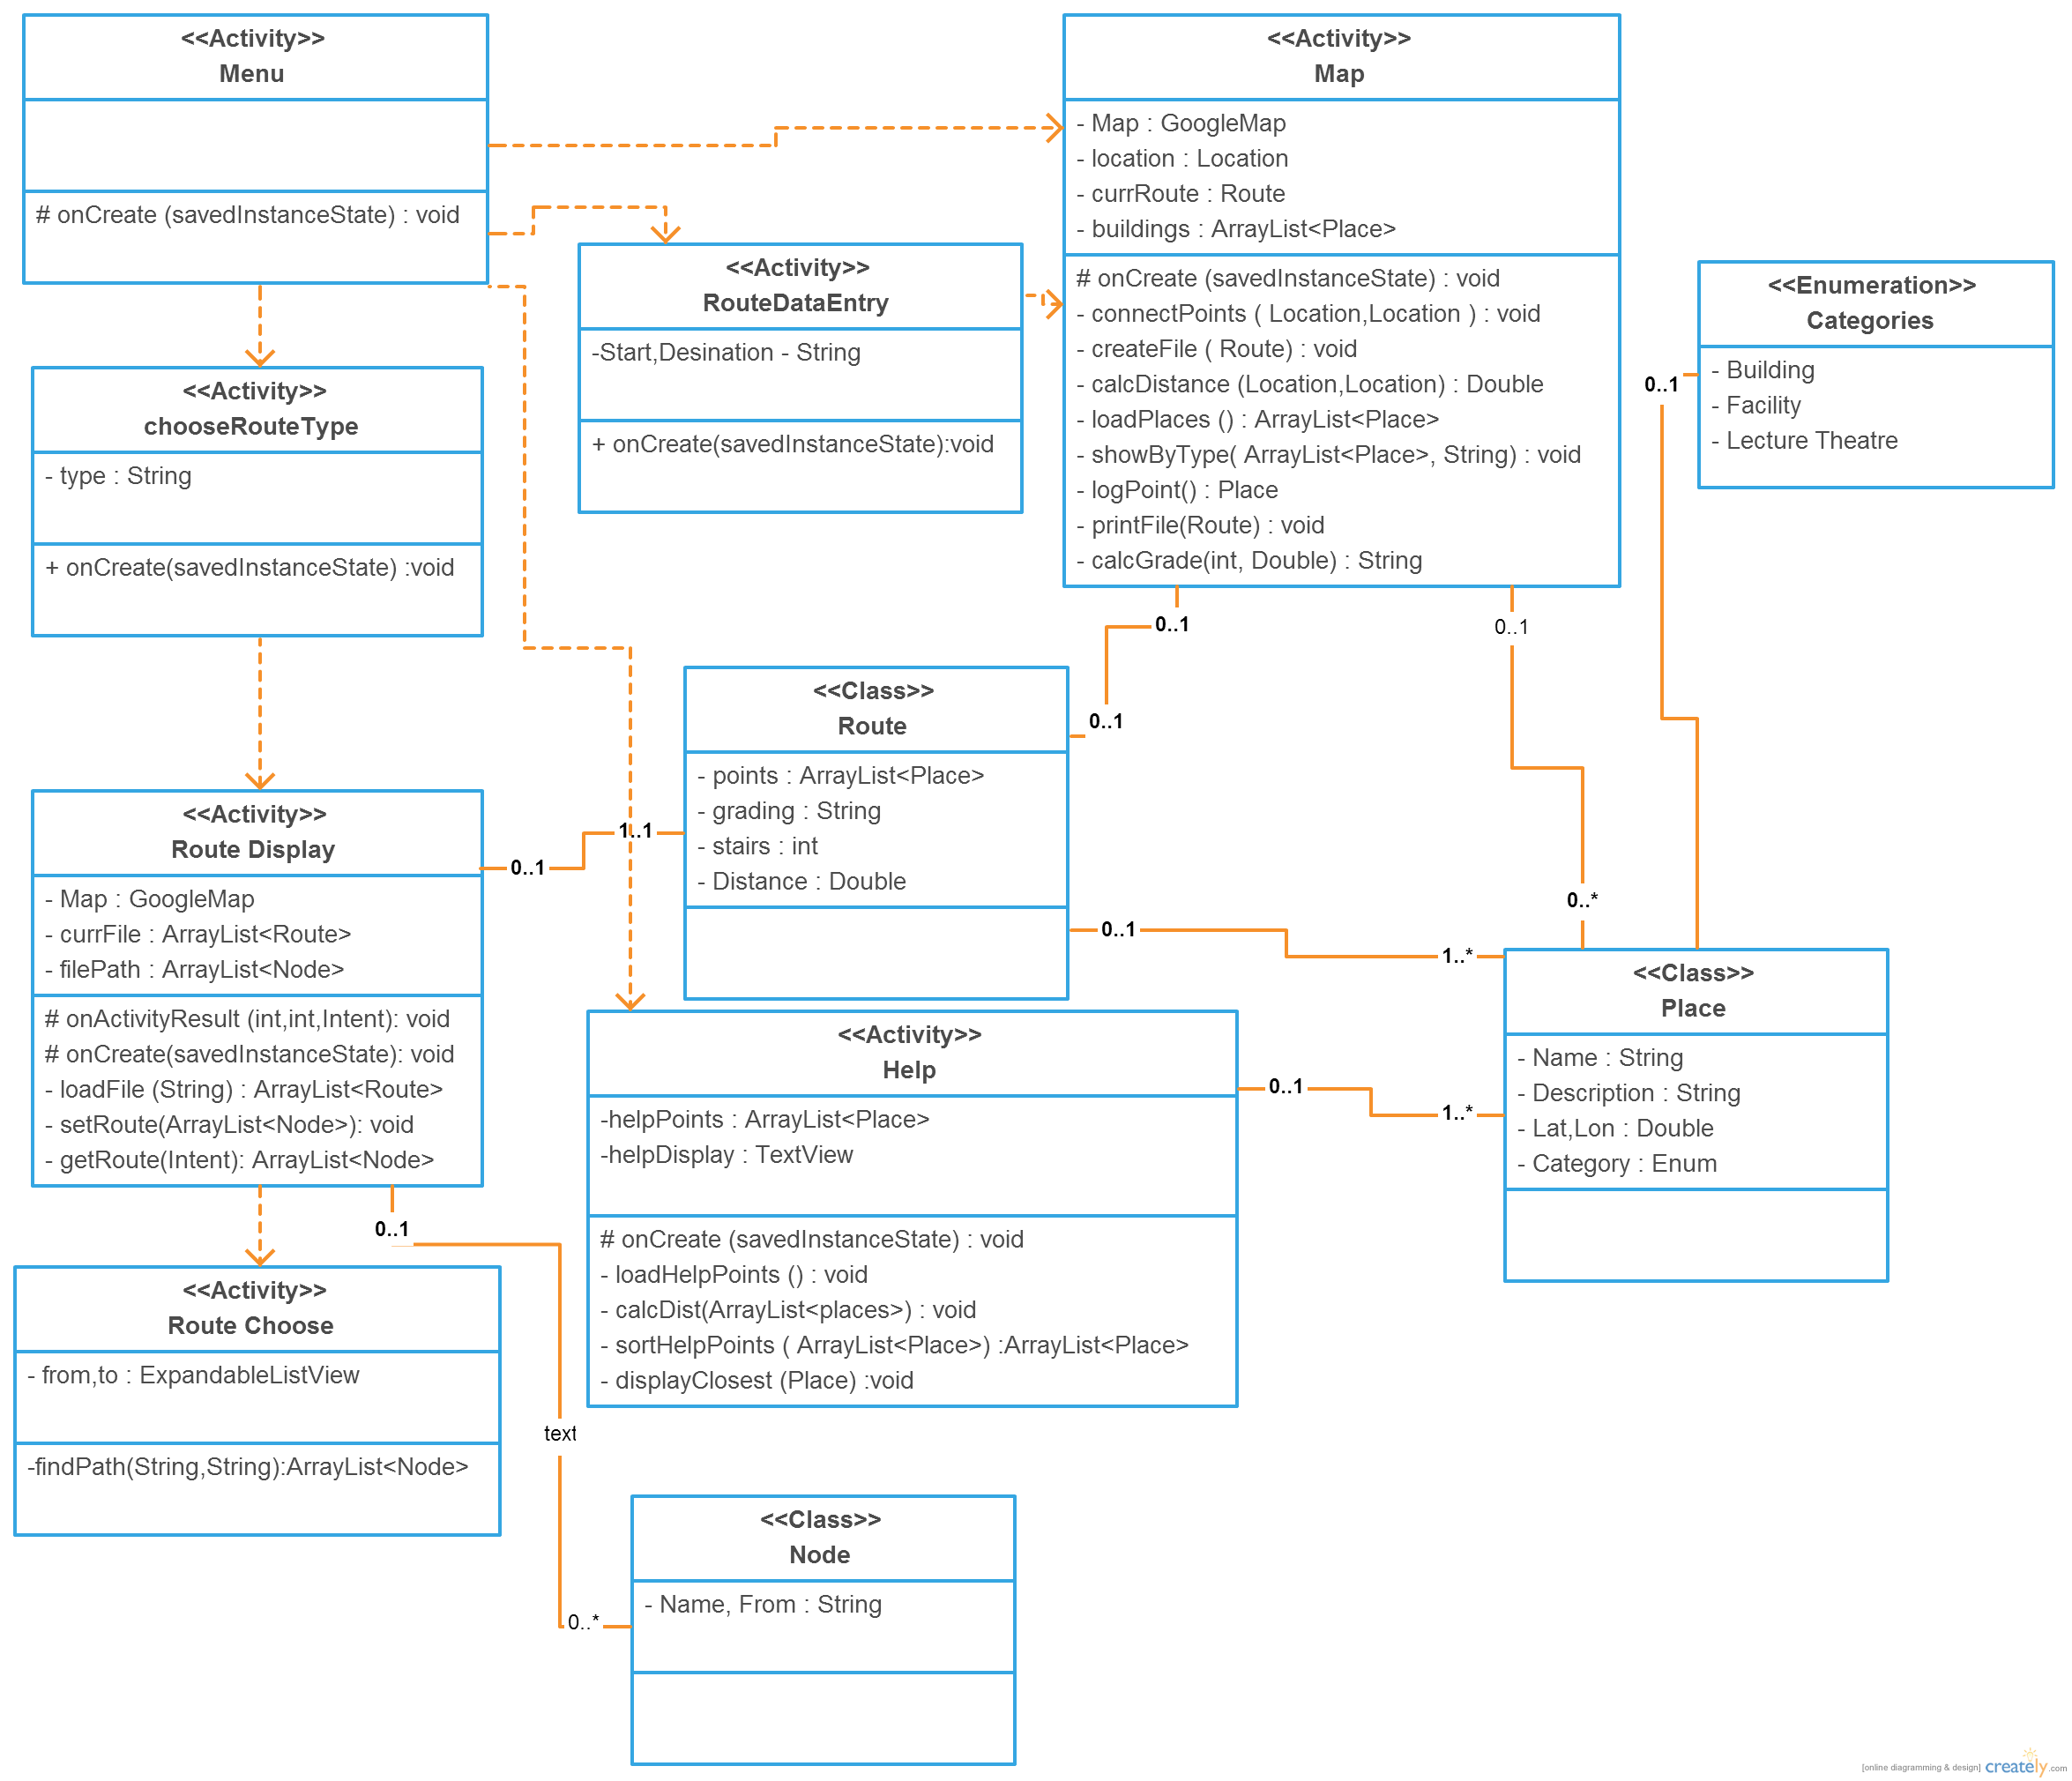
\includegraphics[scale=0.25]{Chapter2/class.png} \\
\caption[Class Diagram]{Final Class Diagram depicting the plan of the implemented system in UML notation}
\end{sidewaysfigure}
\newpage
\section{Application Flow}
With this application most users will be first time users, it is not likely it will be repeatedly used by someone after they are used to the campus. With this in mind it becomes clear that good UI design is important, along with logical flow of the application. A basic flow of screens can be seen in 2.2 however it describes a very broad series of events. In this section a detailed flow of data and screens will be detailed to help with the implementation phase. The diagrams following and the textual descriptions should be used as a framework to build around. 
\subsection{Overall Justification}
A similar diagram to this can be seen in the Design Specification, section 4.1, however this revised version details updates including additions of screens and specific details on what should be contained within some algorithms and the alternative considered. 

One of the changes included within this diagram is the inclusion of the Route Data Entry Activity, this is used for the user to enter the start and destination of the route they are plotting. While this obviously needed to be included it was not within the original diagram, a major decision revolving around this screen is exactly where it should be placed within the application. It is viable to include the screen between either the choice and the plotting screen, or have it used after the user chooses to upload the route they are currently plotting. It has been decided to include this before the user plots anything, this is due to to the idea that the user should provide broad details like the start and end before adding information about the detailed route. It follow a logical progression this way. 

After these details are chosen the $addInfo()$ and  $renderPlotter()$ functions are run. These should actually be run in the $onCreate()$ within the Map Activity. This way the information added in can be accessed from the past Intent to detail what to render and what to name the route. This also applies for the $renderDisplay()$ method, the decision on which should be run is actually made in the $onCreate()$ it just makes more sense to draw it as happening before the screen fully exists, which is technically true as the $onCreate()$ method is what is creating the screen. 

Once at the Map activity various methods can be run depending on what was rendered. If the Building Display screen is shown the user can only select the type of a building to show, one type at a time. This has been a feature repeatedly mentioned, the hard decision to make is whether users will want to see multiple categories at a time. Testing after implementation will have to be completed to gather new user feedback as little is mentioned from the original user feedback. With it not being an issue previously it is considered to not be one currently.

If the user has selected to be able to log a point various possibilities become available, the main method being $logPoint()$ which allows the addition of a point, this should use a Location Manager to retrieve GPS co ordinates and add them to both the map and a Route object for printing later. Once a second point has been added, and continually from there, lines should be displayed to visualize the route. This is easily done using a poly line on the Map object and the co ordinates already retrieved. Other options include $cancel()$ which will reset the Route object and call $Map.clear()$ to provide a fresh start. Another decision was made here, it would be possible on cancelling a walk to bring the user back to the data entry screen, however it is being assumed that the user will have got that information right and if not will return themselves, forcing the restart of the whole process is unnecessary. A smaller method is actually the $addStair()$ function, this should be run on the change of a value in the stair counter. It will simply update the value of the stairs in the Route object. 

Finally the $saveRoute()$ function could be called, to print the Route object to a file compatible with the Route finder. Printing the file is fairly simple, it just has to match the format set out for Routes which will be discussed further on. The file should be printed to the devices memory\cite{storage} for access later by the user. A major decision made here, discussed previously in the original Design specification 2.1.2 and here in 1.1.1 , is whether to have it uploaded or just saved, in short internet on campus is not always available so the decision has been made to save locally to avoid problems relating to communications. Saving the route should also provide a grading, this will be decided through a small formula which considers total distance covered between points and the steps added on the route. 

Most information on the Help section of the application has been discussed previously in Design 4.2.1. It is a fairly simple process, loading in help points and finding the closest using the $greatCircle()$\cite{circle} function. However a further design decision has been made which is hard to represent visually. This is if the value should be updated past the first run, whether the help screen should change while the user walks around with it open. However this idea has been omitted due to the problems and uncertainty it causes, if the method is run every ten seconds for an update, poor GPS signal could mean that when around the boundary of a help point the wrong one is shown occasionally causing confusion. To combat this it would mean taking a set of co ordinates over a time span and finding an average using them, giving a more accurate figure. However it has been decided to just use the first reading, GPS is mainly reliable\cite{accuracy} and the problem revolving around a boundary is unlikely to appear, most people will be well within a building when they need help, not outside and close to another with a help point. 

By far the most complex feature in the application is the route finder and a great deal of thought has gone into how to configure the set up to fit into what the developer thinks is possible during the design phase. While there are many ways to implement what is done, an affecting factor was always the extendibility of the project. At completion the project should have many open ends within it, to allow for the addition of further graphs,locations and make the editing of menus easy. 

In the flow diagram the user is initially sent to the Route type activity, this should allow the user to choose between two separate modes, the step free mode or the standard mode. Step free will be a graph that has been built that avoids stairs. While it would be possible to build a more complex base graph and further change the algorithm the problems these implementations pose could create time restrictions on other areas of the project. Once chosen the type will be saved by the Route Display activity. 

Once at the Route Display activity initially just a map of Aberystwyth and the campus will be shown as no route has been selected, the user should have to click a button to be taken to the Route Choice activity. On this page Expandable List Views should be used to simplify the route selection process, these should then be populated from a text file to help with addition of locations further on. After the user has chosen there locations, feedback should be provided on the page of exactly which locations are to be currently used. Giving feedback to the user through the entire project is key, something that will be discussed further in the design section. 

Once these have been chosen the Breadth First Search will be run to find the path, further details provided in section 2.5. What is likely to happen is that the algorithm will find a set of paths rather than one, these set of paths will build to link a full route from the start to the destination. Implementing the system in this way fixes the problems with the maintainers having to add hundreds of routes just to add a new location, in this version all that has to be built in is one new route connecting the graph to the location and vice versa. 

Plotting the route is seen as a separate task to finding it, finding a path through a graph will end with us just knowing the last accessed node which opened the destination. From there we need to plot backwards from the end. Moving through the nodes based on what location opened another should allow us to move backwards from the end node to the start. This also gives us the smaller routes to plot to display the full route to the user.

Painting the route is then fairly simple, we know which location opened another so we can just search for that locations file and paint the single route to the next one. Repeatedly doing this for each node until the destination should lead to the full route being displayed to the user.

Some consideration should be made to logging a users location on  the route and showing it to them, however this can be enabled through the use of a Google Maps API method called $setMyLocationEnabled(boolean)$\cite{setlocation} which should give us the required effect. From there this can be customised to provide the user with more information than a dot. 

\begin{sidewaysfigure}
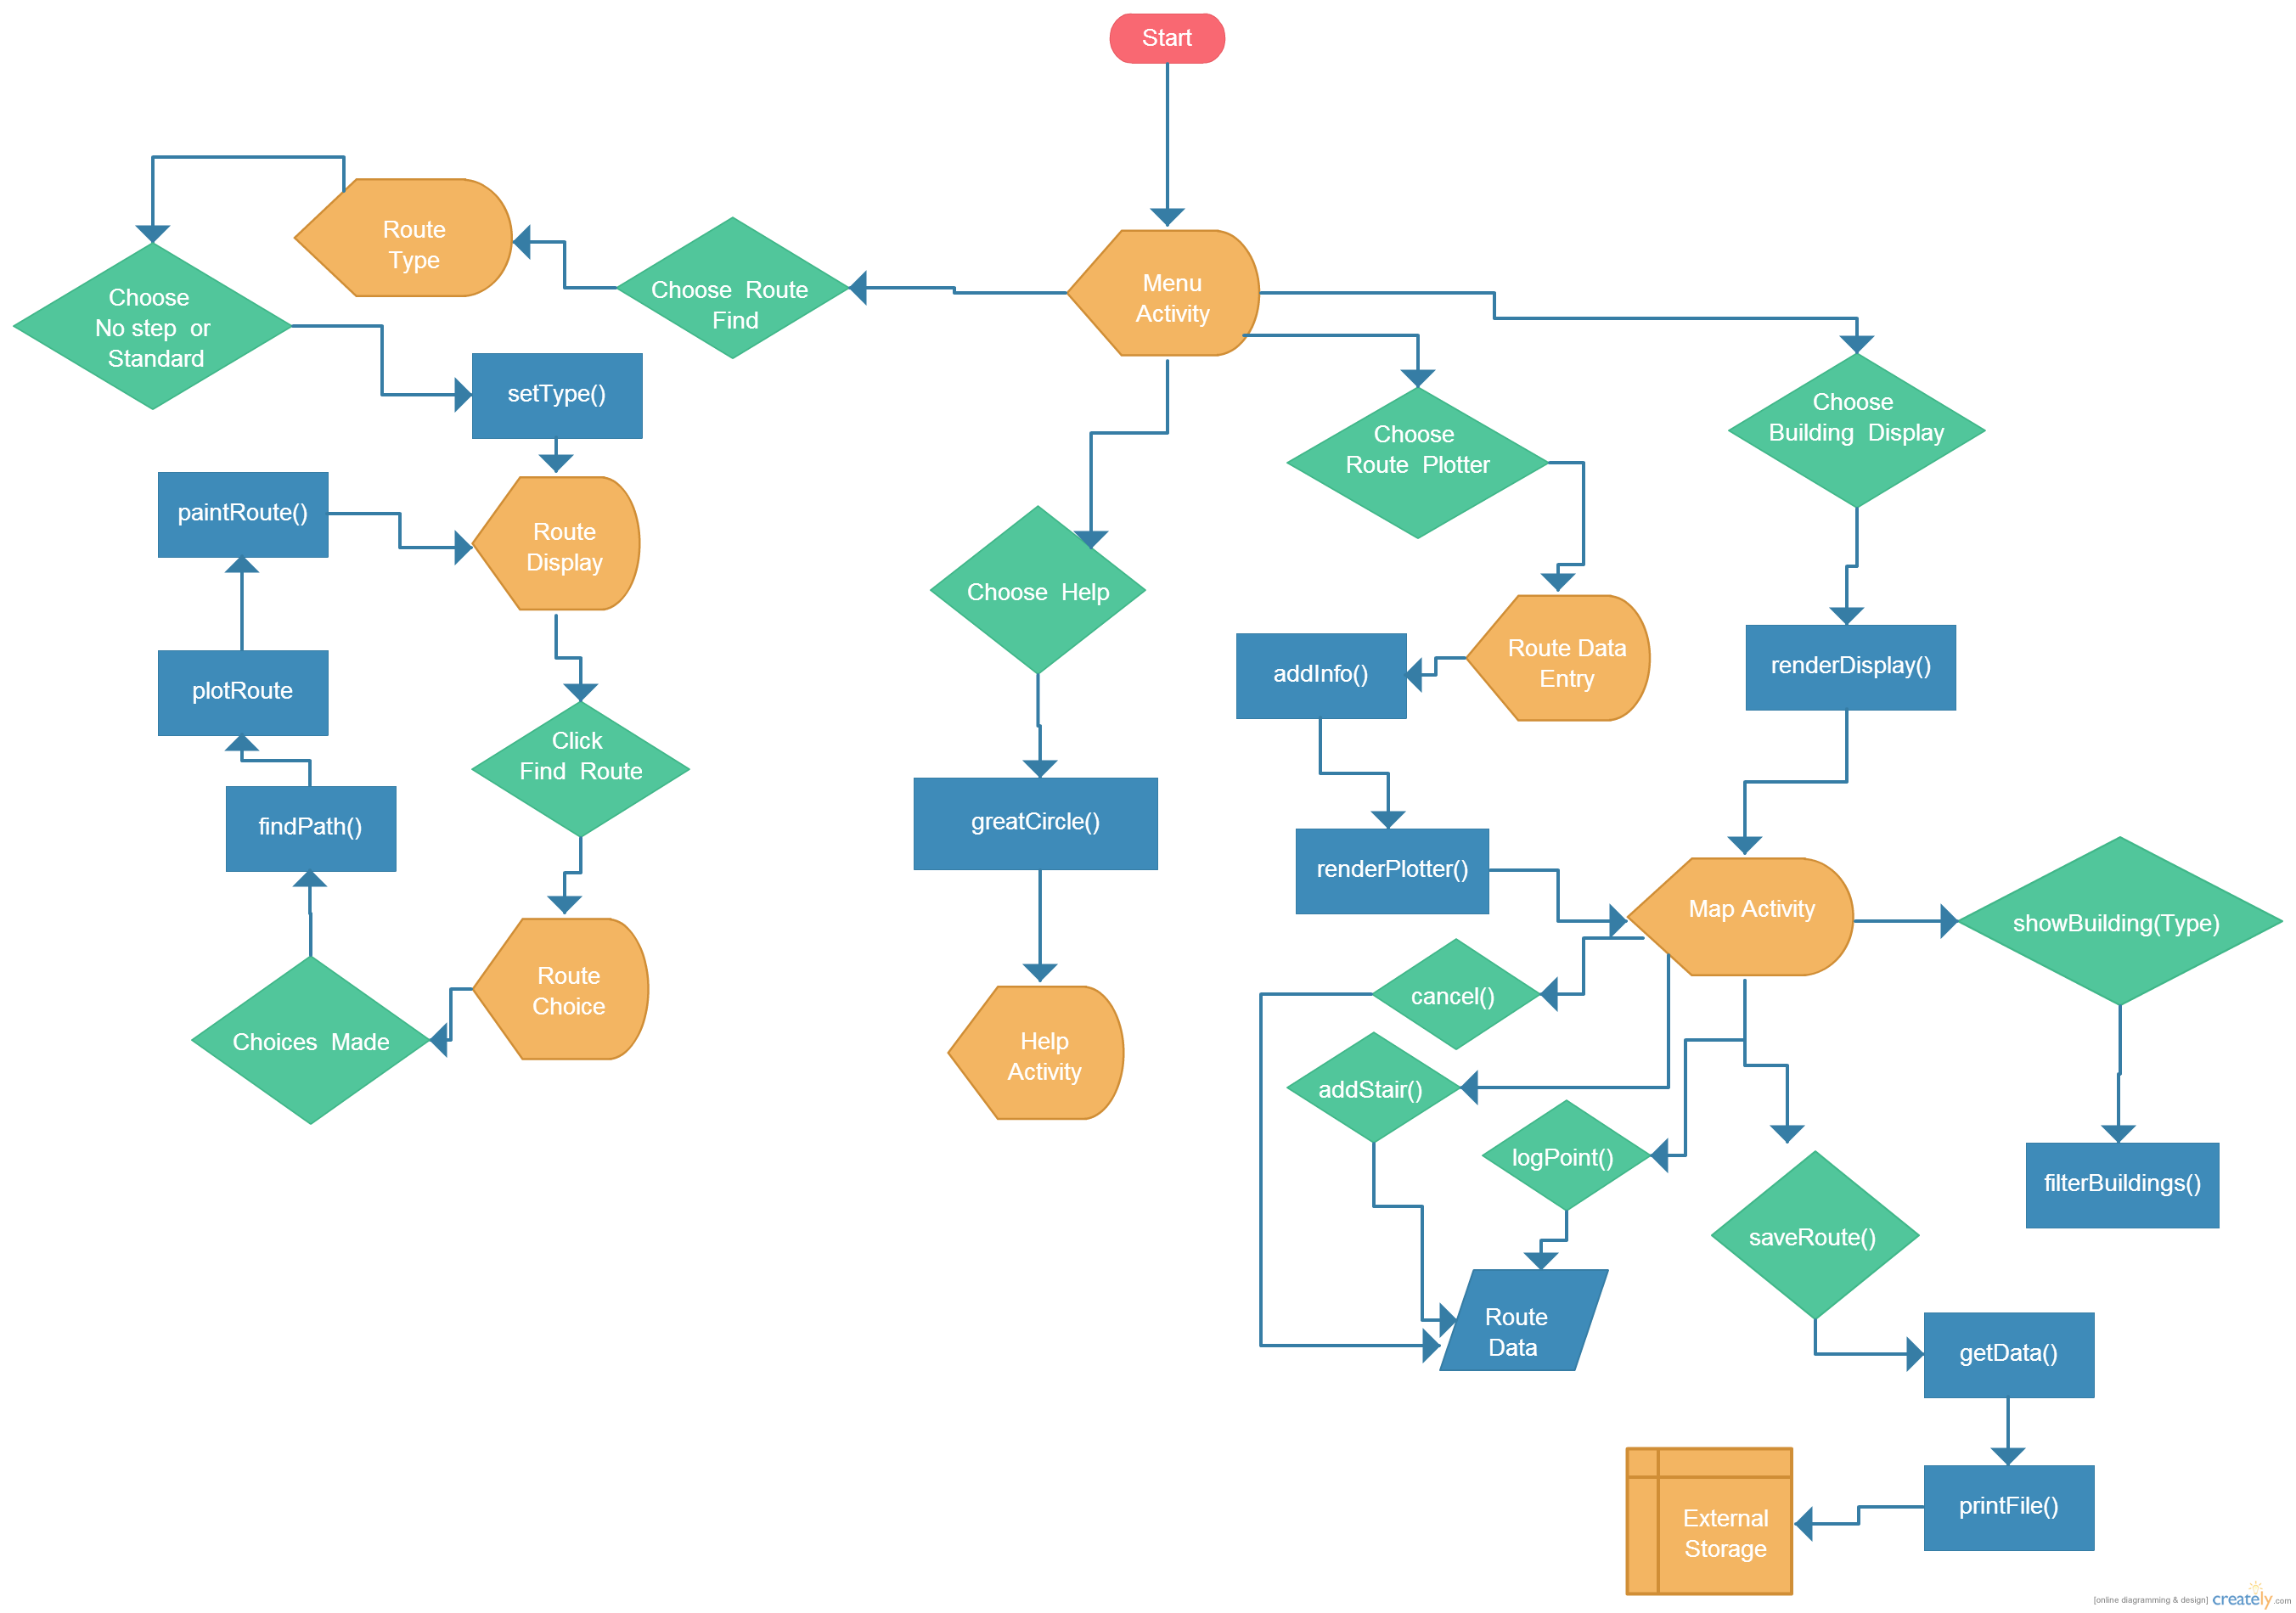
\includegraphics[scale=0.22]{Chapter2/flowo.png} \\
\caption[Flow Diagram]{Current Flow Diagram depicting the flow between screens and processes within the program}
\end{sidewaysfigure}
\newpage
\section{Sequence Diagrams}
\section{Major Algorithms}
Throughout the application there are thought to be a range of major algorithms, most of these relate to the finding of a route and then the visualizing of that route. Currently the algorithm is expected to be a version of BFS when required to go past a single connecting node. Past designs of these algorithms can be seen in Design Specification 3.3. Following are the currently expected algorithms to find routes, calculate distance and read in the file format.

Initially route finding was shown in a single algorithm which is mostly correct, however due to the files containing all of the routes from a point the process has been changed. Initially a check will be made to see if there is a direct connection between start and end, if not then the BFS algorithms will be called. To start the algorithm should look as follows, this should check the original nodes connecting nodes. It logs the connecting nodes and if none are the destination they will be passed to the $deepFind$ which is the BFS. 

It does this by using a boolean which is changed on a route being found. At the start of the BFS it should be noted that the start node, which will be stored in the activities variables, should be added to the visited list to avoid the nodes checking that. 
\vspace{0.3cm}
\hrule
\vspace{0.1cm}
\textbf{Find Initial Path}
\vspace{0.1cm}
\hrule
\vspace{0.1cm}
\begin{algorithmic}[1]
\State$startRoutes$ = read($start$)
\State $found$ = 0
\State ArrayList $routeEnds$
\For{$startRoutes$}
	\State $routeEnds$ add $route -> end$
	\If{$route -> end = end$}
		\State Plot Single Route $route$
		\State $found$ = 1
	\EndIf
\EndFor
\If{$found == 0$}
	\State deepFind $routeEnds$
\EndIf
\end{algorithmic}

The deep find algorithm will initially be a BFS, a mostly correct version can be seen within the Design Specification however it does not account for being passed it starting nodes. The actual implementation should look close to the following pseudo code. 

In this example you can see that the start node is set to visited and the nodes to be cycled through as those passed in as a variable. While the algorithm looks relatively simple set like this due to having to implement loading from the devices memory and other functions it is expected to take time to develop. Initial research has been conducted on loading. 

A key line which helps in a later algorithm can be seen on line 11. This helps us move backwards from our destination as we can tell which connecting Node each Node was opened from, essentially plotting the path backwards by tracing the algorithms steps. 

In future it is advised that more complex search algorithms are considered, including A*\cite{astar}, to try and find a more efficient algorithm as on a large graph BFS could cause a small delay on older mobile devices. 
\vspace{0.3cm}
\hrule
\vspace{0.1cm}
\textbf{Find Route}
\vspace{0.1cm}
\hrule
\vspace{0.1cm}
\begin{algorithmic}[1]
\State $start$ set Visited
\State $Nodes$ = $passedInNodes$
\While{!route found} this
\For{$Nodes$} 
\If {$Node$ has been visited}
    \State do nothing
\Else
	\State set $Node$ visited
    \State get $Node Routes$
    \For{$Node Routes$}
    \State Set Opened from $Node$
    	\If {$Node Route End$ = Destination}
    		\State set route found true
    		\State call Plot Path ($visited$)
    	\EndIf
    	\If {$Node Route End$ not visited}
    		\State Add to Nodes
    	\EndIf
    \EndFor
\EndIf
\EndFor
\EndWhile
\end{algorithmic}

As can be seen in the above algorithm the visited nodes are passed in as a variable to the function that will plot the path, this way access is provided to the information about which Node was opened from where, allowing the function to work backwards though the Nodes.

This is possible due to the fact that as soon as a single route is found that connects to the end no more are looked for, by doing this we guarantee only one path being painted. However this plan does not work if the search finds multiple paths, something that needs to be noted for future development. 

Due to the nested loops the algorithm should always paint all required routes. 
\vspace{0.3cm}
\hrule
\vspace{0.1cm}
\textbf{Plot Path}
\vspace{0.1cm}
\hrule
\vspace{0.1cm}
\begin{algorithmic}[1]
\State $Visited Nodes$ = $visited$
\State$search$ = destination
\For{$Visited Nodes$}
	\For{$Visited Nodes$}
	
	\If{$search = Node Name$}
		\State Plot Single Route 9$Node->name, Node->from$
		\State $search = Node from$
	\EndIf
\EndFor
\EndFor
\end{algorithmic}
Pseudo code for plotting a single route and then painting it can be found in the Design Specification sections 3.3 and 3.4. These have not changed through further design and are expected to suffice as they are. This also applies to the saving of a route file algorithm, found in section 3.5. However after research it has been noted that external memory is not always provided and as such further checks should be completed\cite{storage}, following example code from both the Android API and other sources\cite{check} it is expected the following code should suffice. 
\vspace{0.3cm}
\hrule
\vspace{0.1cm}
\textbf{Check State}
\vspace{0.1cm}
\hrule
\vspace{0.1cm}
\begin{algorithmic}[1]
\State $state$ = $getExternalState$
\State $possWrite$ = false
\If {$state$ = $readOnly$}
	\State Cannot create files
\ElsIf{$state$ = $readWrite$}
	\State $possWrite$ = $True$
\Else{}
	\State Something is wrong, we only have one desired result which we have checked for
	\EndIf
	\State return $possWrite$

\end{algorithmic}
An algorithm which has been previously overlooked as it was initially assumed to be fairly simple is the file writer. After further research which resulted in the memory check algorithm\cite{check} it has been decided that its process should be noted due to the various ways it could be completed. A further decision which has been made is to include the saving of a file into the file writer function, this way when a user initially goes to save a file the folder will always be present. Initial design should be as follows. 
\vspace{0.3cm}
\hrule
\vspace{0.2cm}
\textbf{Save File}
\vspace{0.1cm}
\hrule
\vspace{0.1cm}
\begin{algorithmic}[1]
\State $root = get Memory$
\State $My Directory = root/routes$
\If{My Directory exists}
	\State Do Nothing
	\Else
\State Make Dir $->My Directory$
\EndIf
\State New File$-> root$

\State $out = Output Stream -> File$
\State $out -> Route ->Start$
\State $out -> Route -> End$
\State $out -> Route -> Grading$
\For{$Points$}
	\State $out -> Point i$
\EndFor

\end{algorithmic}
\section{Interfaces}
User Interface was an area in which the developer had little to no experience, while basic GUI's had been developed before they did not truly consider a users habits and motivations. From the initial design specification to the beginning of implementation research was completed on both good design guidelines and the options provided through Android and its use of XML for layouts. 

While UI was seen as a less important task than the actual underlying code a set of basic rules were set out from the start, taking influence from other applications and the Google Material Design outline\cite{material}. While the material design outline was not adhered to fully it provided good insight on the vision Google has for the Android platform. 


\begin{itemize}
	\item 1 - Make best use of white space within design, make it act as a barrier rather than having to add an actual barrier in.
	\item 2 - Bold colours will help cause distinction between background and active UI members.
	\item 3 - Theme should be carried throughout pages as best possible, little to no room for exceptions. 
	\item 4 - Develop a system which supports the same experience throughout devices. XML allows for relative layouts so no fixed measurements mostly. 
	\item 5 - Interactive elements need to be responsive, users need feedback on their actions. This can be textual or a change in colour. Noise is not practical. 
\end{itemize}
\newpage
\subsection{Colour Theme}
Colour theme was something that the developer felt was key to a successful UI, without it a good layout would go to waste. Due to this several sets of colours were chosen at the start for trial upon the full completion of the application. Intially design highlighted a yellow and purple theme as the likely choice, due to matching the universities website. However as design furthered and prototypes were developed of basic layouts, it became obvious this may not be the ideal theme. These themes were both developed internally and taken from on line resources. The following were chosen due to them being seen as palettes that would not only provide good distinction between members of the UI but provide an easy to view screen. Using many bright and clashing colours could possibly create a visually offensive UI which is something to be avoided. By using safe, strong colours a higher chance of success was predicted. 

\begin{figure}[h]
1.

\includegraphics[scale=0.5]{Chapter2/colourone.png} \\

2.

\includegraphics[scale=0.5]{Chapter2/colourtwo.png} \\

3.

\includegraphics[scale=0.5]{Chapter2/colourthree.png}
\caption[Theme Possibilities]{Theme Possibilities that could be applied to the application}
\end{figure}
As visible from the above diagram the palettes were based on what seemed to be sequential colours as such, while no actual math was applied to come to this decision it was visually apparent that the themes were a progression of shade. However this provides the developer with a range of possibilities, with the shades being far enough away from each other, text of one colour should always be visible on another due to the lack of overlap. It is advised during development though that text of one colour be on the background of a colour at least one away. 

For example, text from the middle of the first palette should only be applied to backgrounds of the two ends, while viable to put on the two connecting colours the impact of the distinct colours will be lost slightly. 
\begin{figure}

\includegraphics[scale=0.5]{Chapter2/textone.png} \\

\vspace{0.2cm}

\includegraphics[scale=0.5]{Chapter2/texttwo.png} 
\caption[Button Examples]{Demonstration of coloured buttons using the possible colour schemes}
\end{figure}

\newpage
As can be seen in the Theme Possibilities above  the principle of using five progressive colour should provide us with a theme that is not only easy on the users eye but provides us with the ability to give a good distinction between UI members and blank space. With the above three options to be tested it is likely that either 1 or 2 will be the final theme. With 3 being viable the colours seem to be bland, while it could work with the right arrangement it is suggested more effort be put into a functional theme built of 1 or 2. 

A similar palette to that of 2 can be seen at outlook.com\cite{out}. In this design the colours are fairly similar with white acting as the background and then a colour similar to the middle acting as interactive elements. Distinction between the two can clearly be seen and as such they stand out as having a purpose, it also helps with the clear display of text while removing cluttering multiple colours may cause. In the design responsiveness is achieved through a brief colour change in the element, something that should be considered within this project. Other considerations to be made in terms of colour design is the implementation of themes for colour-blind users, however this a stretch goal and unlikely to be implemented. 

Mock up screens of the application with the prospective colour schemes can be seen below, with these it is is clear to see why 1 and 2 have an advantage over 3. It should be possible in future for the user to define a theme from a set of options, not only will this help users who make frequent use of the application but it will provide a way for the colour-blind themes to be implemented without a separate application. \\
\begin{figure}
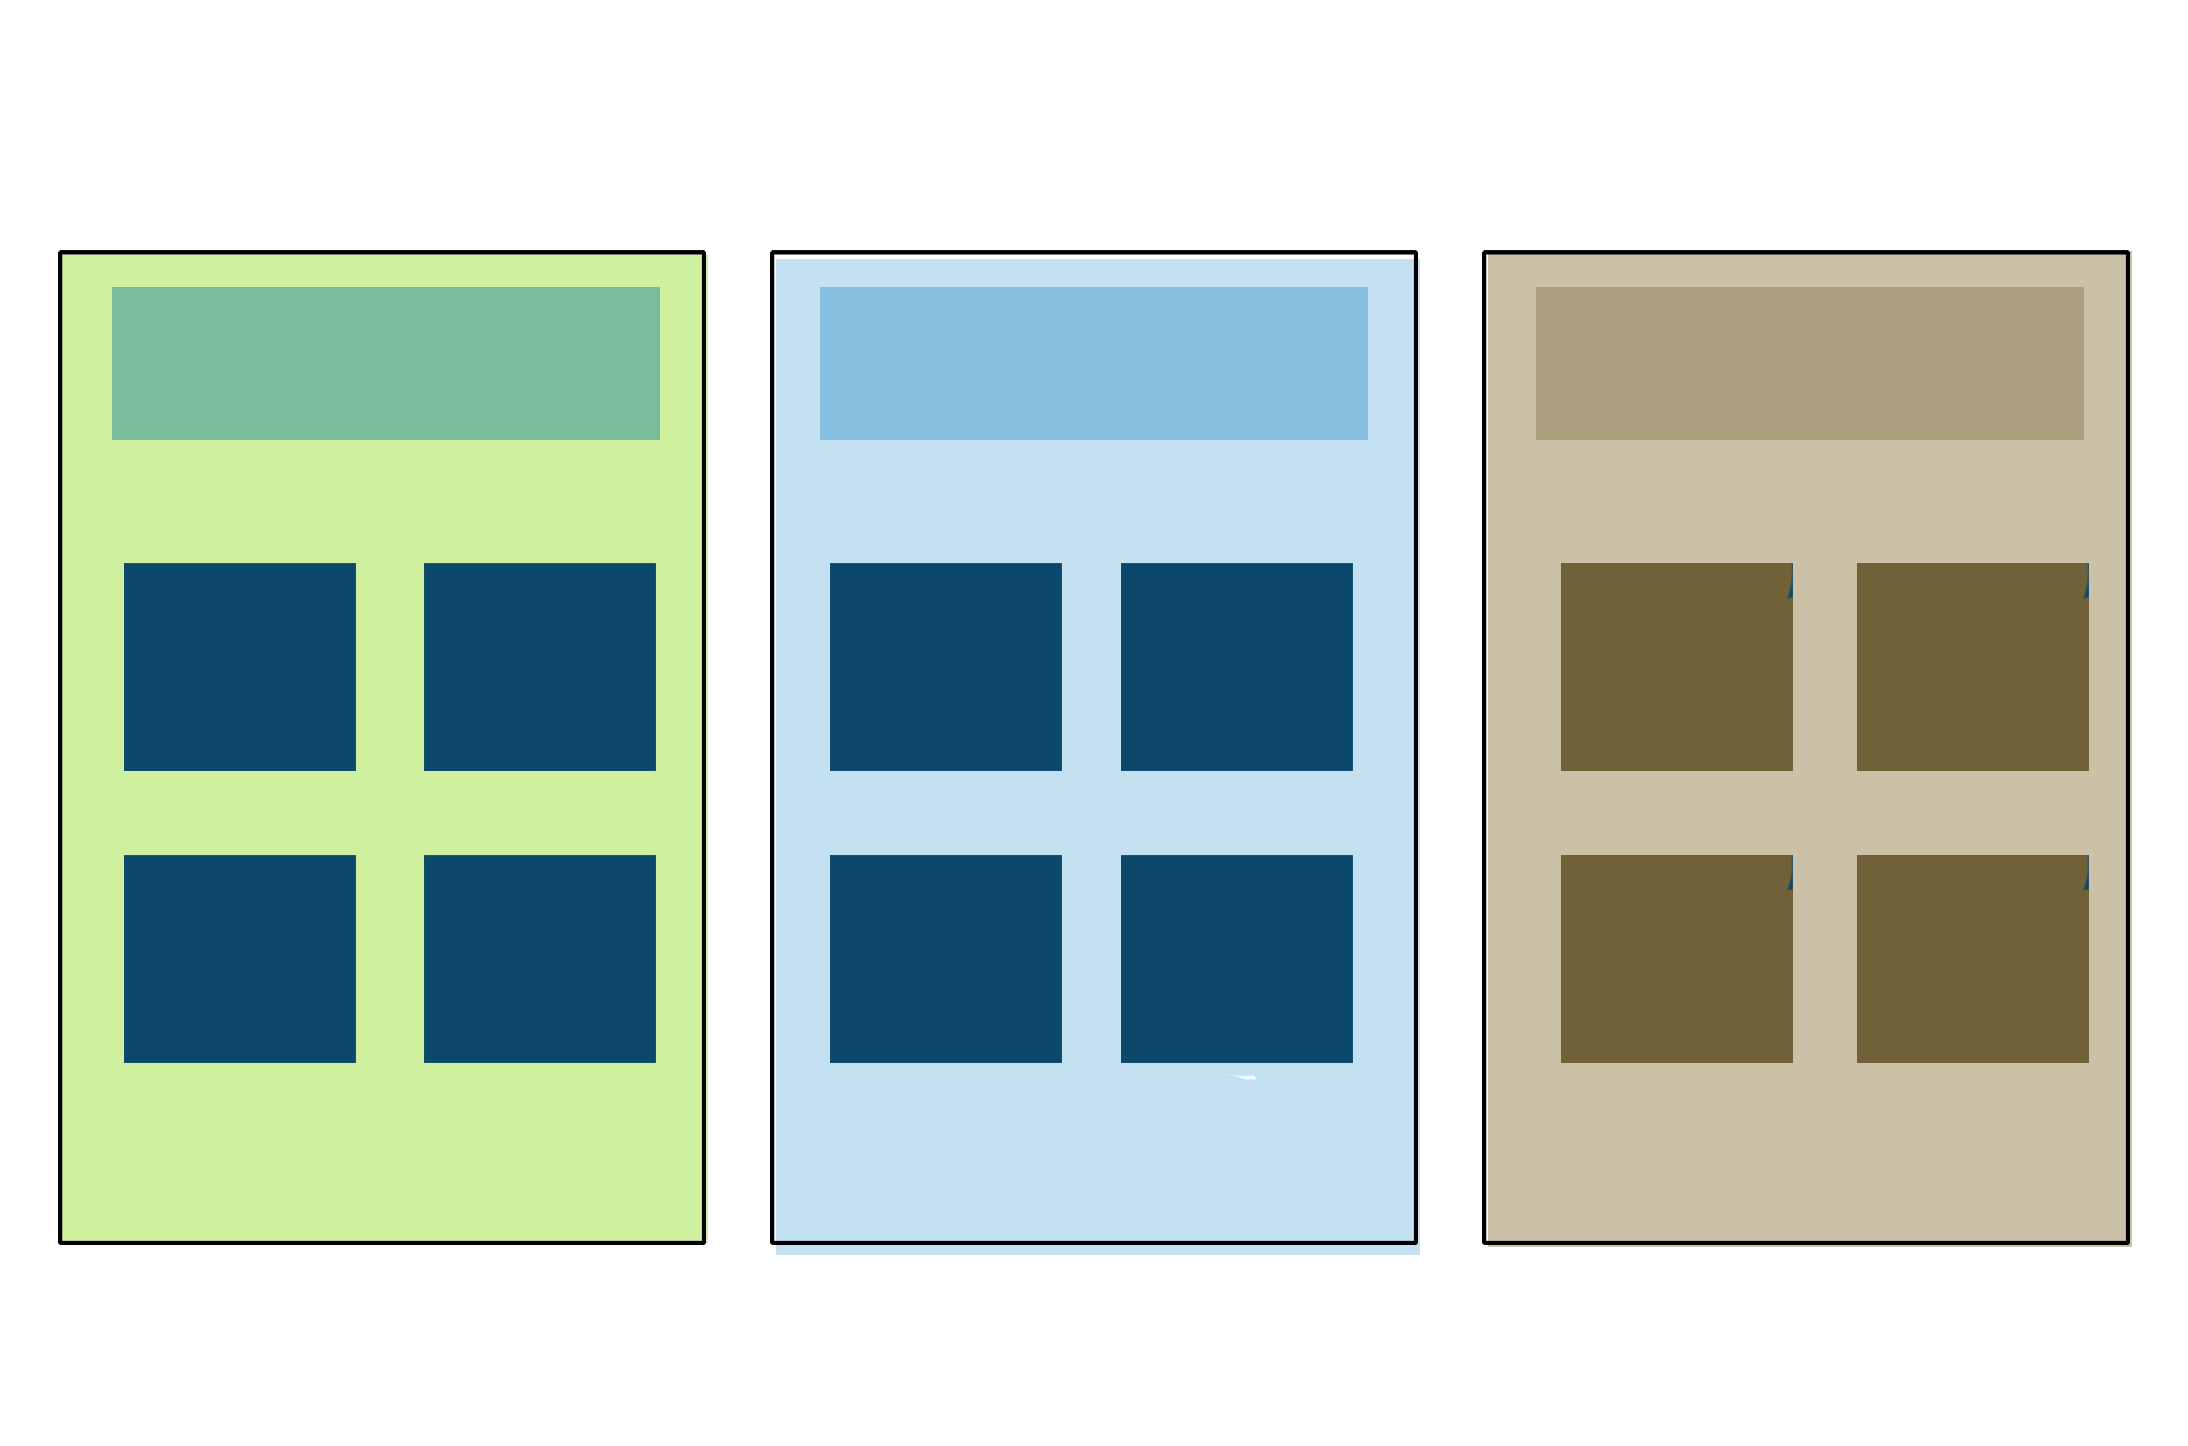
\includegraphics[scale=0.7]{Chapter2/themes.png} 
\caption[Example Themes]{Example Themes demonstrated as to how they would look on the application}
\end{figure}

As it stands theme 1 is seen to be the most likely candidate, it provides a range of sequential yet clearly varying colours that do not look quite as unvarying as the other two options. With this visual representation it is clear to see why option 3 is unlikely, however with the use of white space it could be a viable option. Colour theme is an area that will have to be tested with the help of human users, response to a design is not something we can simulate. By completing tests on actual users not only can we plot out the decision making and adapt around it, we can get feedback on clarity, simplicity and overall operability. A fully working application that a user can easily navigate through is the prime objective of this project. 
\subsection{User location}
Display the users location to them is seen as a key element to route finding, displaying a route is only so much use if a user cannot see where they are on it. While the solution to this problem has already been discussed, some additions can be made to it. Mainly the addition of custom graphics to benefit the user. 

This is something which is covered on the introduction page to the Maps API\cite{maps}. From that and some basic research it is possible to see that custom graphics and a movable camera are both possible. Giving the developer to implement an almost sat-nav feel to the application. 

A range of graphics have already been drawn up to discuss possible implementations of the 'arrow'.

As can be seen from the above diagram, 1 which is a representation of the basic user location does not really provide the user with too much information, it will sometimes change based on a users direction but the feedback is not obvious and those with poor vision may not be able to notice it at all. 

Possible graphic 2 is the most likely option, along with 3. These two implementations of the arrow system show the user there direction and close location without too much hindrance to view or complications based on confusing graphics. It is advised that if 2 is implemented it be made to be clearly separate from the map, while unlikely to be mistaken for a map feature a bad implementation would still allow for the possibility. Option 3 avoids this problem due to the containing circle.

Option 4 is an adapted version of 1, with the direction being clearer and as such would likely be an improvement. However with the viability of 2 and 3 being much higher it is unlikely that it will be chosen.

The theme for the guidance will follow whichever is chosen by the developer for the overall application. Creating a familiarity between the user and what they are being shown, if all interactive elements are previously shown in one colour then the arrow should follow, making it recognisable as something that will change or provide assistance. 
\subsection{Screen Designs}
Some initial screen designs can be seen in the original Design specification, while rough there overall display will not be altered too much for the development. However the theme used and some of the options made will make it hard for the screens to be implemented as they are on various screen sizes, especially on the menu screen.

In the original designs the Menu Activity is shown as a screen with a list of buttons which would then link the user to the respective Activity. However, on multiple screen sizes the buttons could start to look like they were rushed due to them just being in the middle, especially on larger screens. Due to this the decision has been made to implement a grid system on the main menu, by doing this we can make the segments relative to the screen and have them fill it. White space should also be left between the segments to provide clear non verbal instruction that the buttons are separate and interactive. 

Further changes include the addition of several screens which were not identified during the start of the project. First of these being the Route Type Activity. In this activity the user is given a choice between the two types of graph they can choose to find routes through. Following is a representation of what should be a fairly simple screen.

\begin{figure}[H]
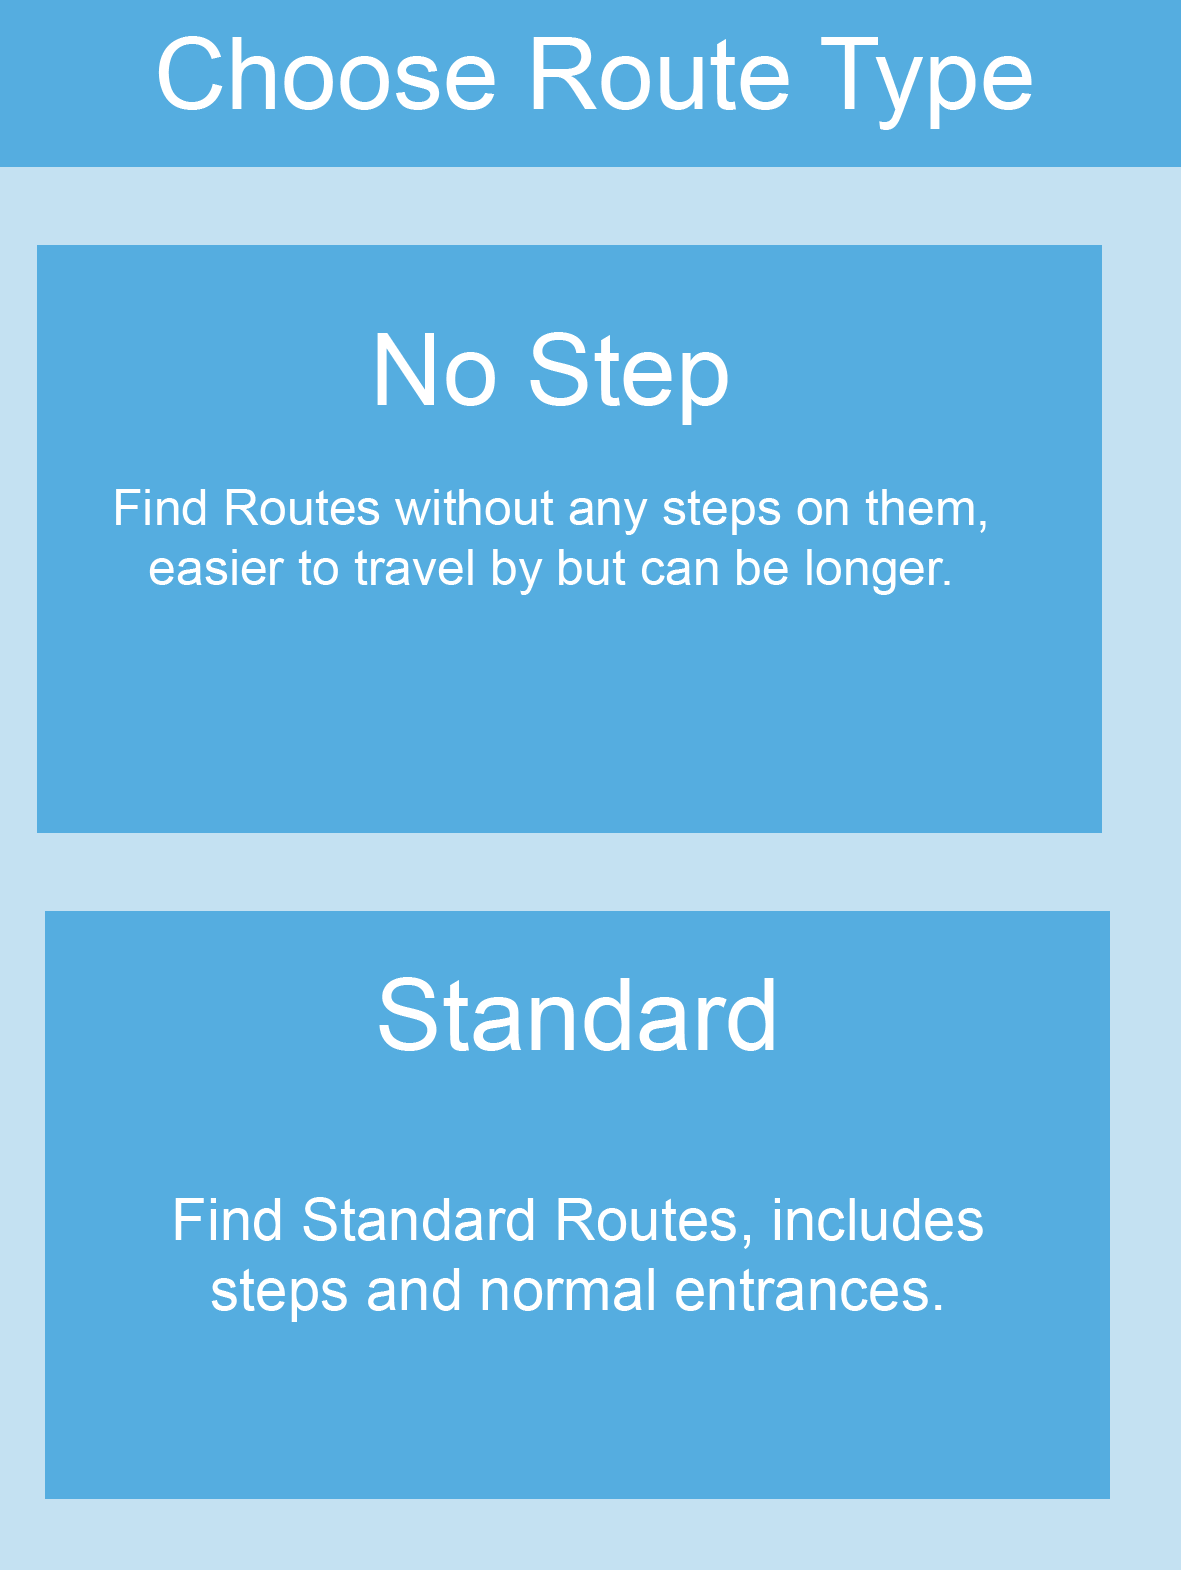
\includegraphics[scale=0.5]{Chapter2/crt.png} 
\caption[Route Type Example]{Example design of the the route type selection screen, final will be either identical or a close variant.}
\end{figure}

Another addition to the set of activities will be the Route Data Entry activity, this will allow the user to enter information about the route they are planning to take. To accomplish this the user should enter the start and end points, from there they can then move onto the actual logging of the route. Again a simple screen due to it being two text entry boxes, only restriction being that of the theme.

\begin{figure}[H]
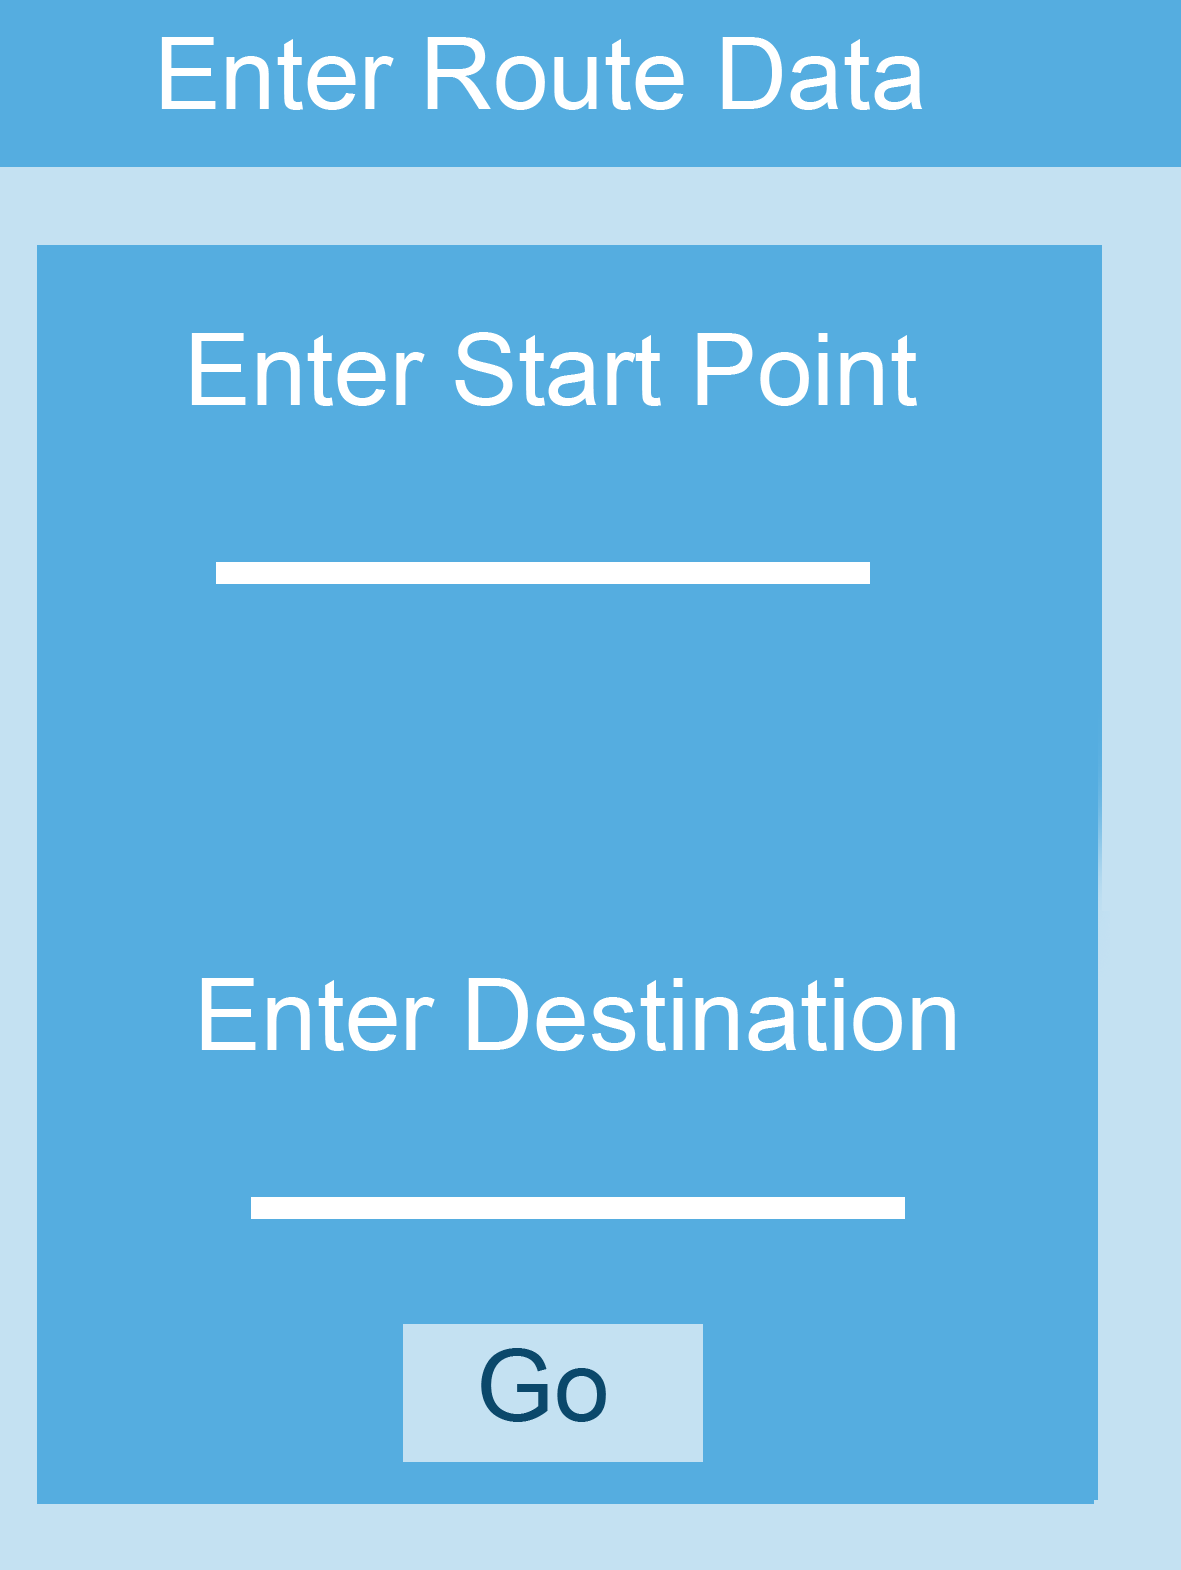
\includegraphics[scale=0.5]{Chapter2/rd.png} 
\caption[Route Data Example]{Example design of the the route data entry screen. Will only be two text entry boxes and a button to proceed.}
\end{figure}
\newpage